\chapter{Casebeskrivelse}
\label{chp:case}
Utbyggingen av det nye universitetssykehuset i Trondheim, St.Olavs Hospital, ble påbegynt i 2003 og sto ferdig sommeren 2013. Byggingen ble hovedsakelig delt i to byggefaser, hvor avdelingene flyttet inn i sine nye lokaler etter hver fase. Som en del av byggeprosjektet inngikk også det som da var Norges største, dyreste og mest kompliserte IKT-leveranse noensinne \citep{TU}. Pasientsignalsystemet var en del av denne leveransen. 

\noindent
Denne casebeskrivelsen omfatter en beskrivelse av de tre avdelingene, A1, A2 og A3, som har vært fokus for forskningsarbeidet. 

\noindent
Med det nye sykehuset ble utformingen av avdelingene endret. Avdelingene er nå delt i sengetun, hvor hvert sengetun normalt har seks til åtte pasientrom. Dette er en fysisk og funksjonell måte å organisere pasientrommene på, og for å sikre fleksibilitet og effektivitet ligger flere sengetun ved en sengepost etter hverandre i serie, som vist i figur \ref{Plantegninger} \citep{Aslaksen, sykehuskart}. Sengetunene består av en arbeidsstasjon, nærlager, sengerom og toalett. Mellom tunene ligger støtterom som kjøkken og oppholdsrom for pasienter, medisinrom, skylle/avfallsrom og undersøkelsesrom. Et overordnet mål for en slik organisering er å redusere barrierer mellom pleier og pasient, bedre muligheter for overvåking av pasienter og redusere risiko for uønskede hendelser, noe som øker sikkerheten for pasientene \citep{Sintef-sengetun}.

\noindent
Avdeling A1 består av tre tun à seks sengerom, hvorav avdelingen har to luftsmitteisolat og seks kontaktsmitteisolat. Avdeling A2 består av tre tun à åtte sengerom. Avdeling A3 består av fire tun à åtte sengerom, fordelt på to etasjer.

\noindent
Avdelingene A2 og A3 er tydelig delt i sengetun (figur \ref{fig:Bevegelse} og \ref{fig:AHL}) mens avdeling A1 skiller seg fra de to andre da rommene er plassert i en lang gang uten tydelig avgrensede tun (figur \ref{fig:Ksenter}). Også utformingen av rommene på A1 skiller seg fra de andre da de har egen luftsluse mellom korridoren og hvert enkelt pasientrom.

\begin{figure}[H]
        \centering
        \begin{subfigure}[b]{1.0\textwidth}
        		\centering
				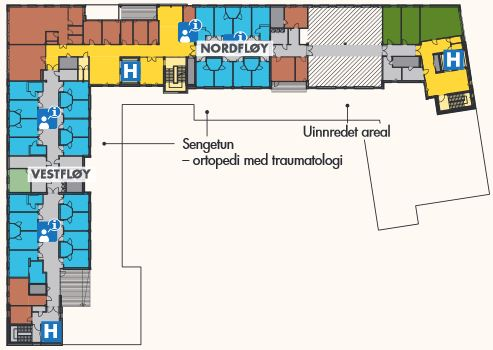
\includegraphics[scale=0.8]{bevegelse_6etg.jpg}
				\caption{Avdeling A2}
				\label{fig:Bevegelse}
        \end{subfigure}
        
        \begin{subfigure}[b]{1.0\textwidth}
        		\centering
				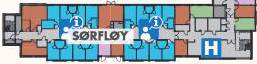
\includegraphics[scale=1.1]{AHL_5etg_sorfloy.jpg}
				\caption{Avdeling A3}
				\label{fig:AHL}
        \end{subfigure}
        
        \begin{subfigure}[b]{1.0\textwidth}
        		\centering
				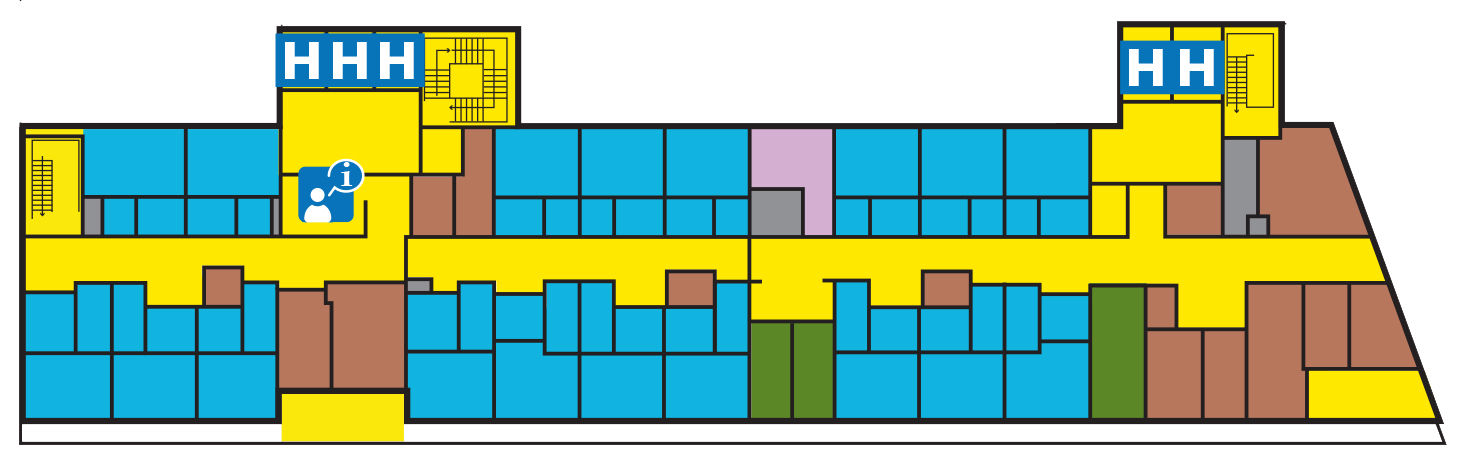
\includegraphics[scale=0.25]{Ksenter_6etg.jpg}
				\caption{Avdeling A1}
				\label{fig:Ksenter}		
        \end{subfigure}
        \caption{Plantegning av avdelingene. \citep{sykehuskart}.}
        \label{Plantegninger}
\end{figure}

\noindent
Arbeidstasjonene er utstyrt med PC'er og fungerer som en desentralisering av vaktrommet. På avdelingene A2 og A3 ligger denne som et senter på det åpne tunet ( figur \ref{fig:aapen_arbeidsstasjon}), mens den på avdeling A1 ligger på rekke med pasientrommene (figur \ref{fig:A1_arbeidsstasjon}).

\begin{figure}[H]
\centering
	\begin{subfigure}[b]{1.0\textwidth}
		\centering
		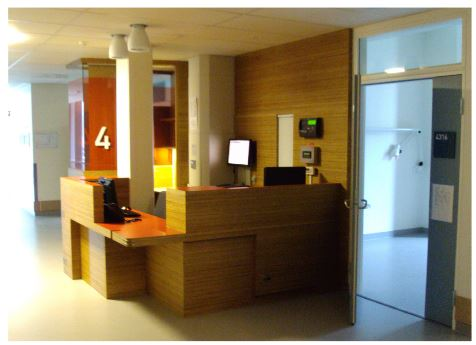
\includegraphics[scale=0.7]{aapen_arbeidsstasjon.jpg}
		\caption{Åpen arbeidsstasjon på sengetun slik den er på avdelingene A2 og A3 			\citep{sykehuskart}}
		\label{fig:aapen_arbeidsstasjon}
	\end{subfigure}
	
	\begin{subfigure}[b]{1.0\textwidth}
		\centering
		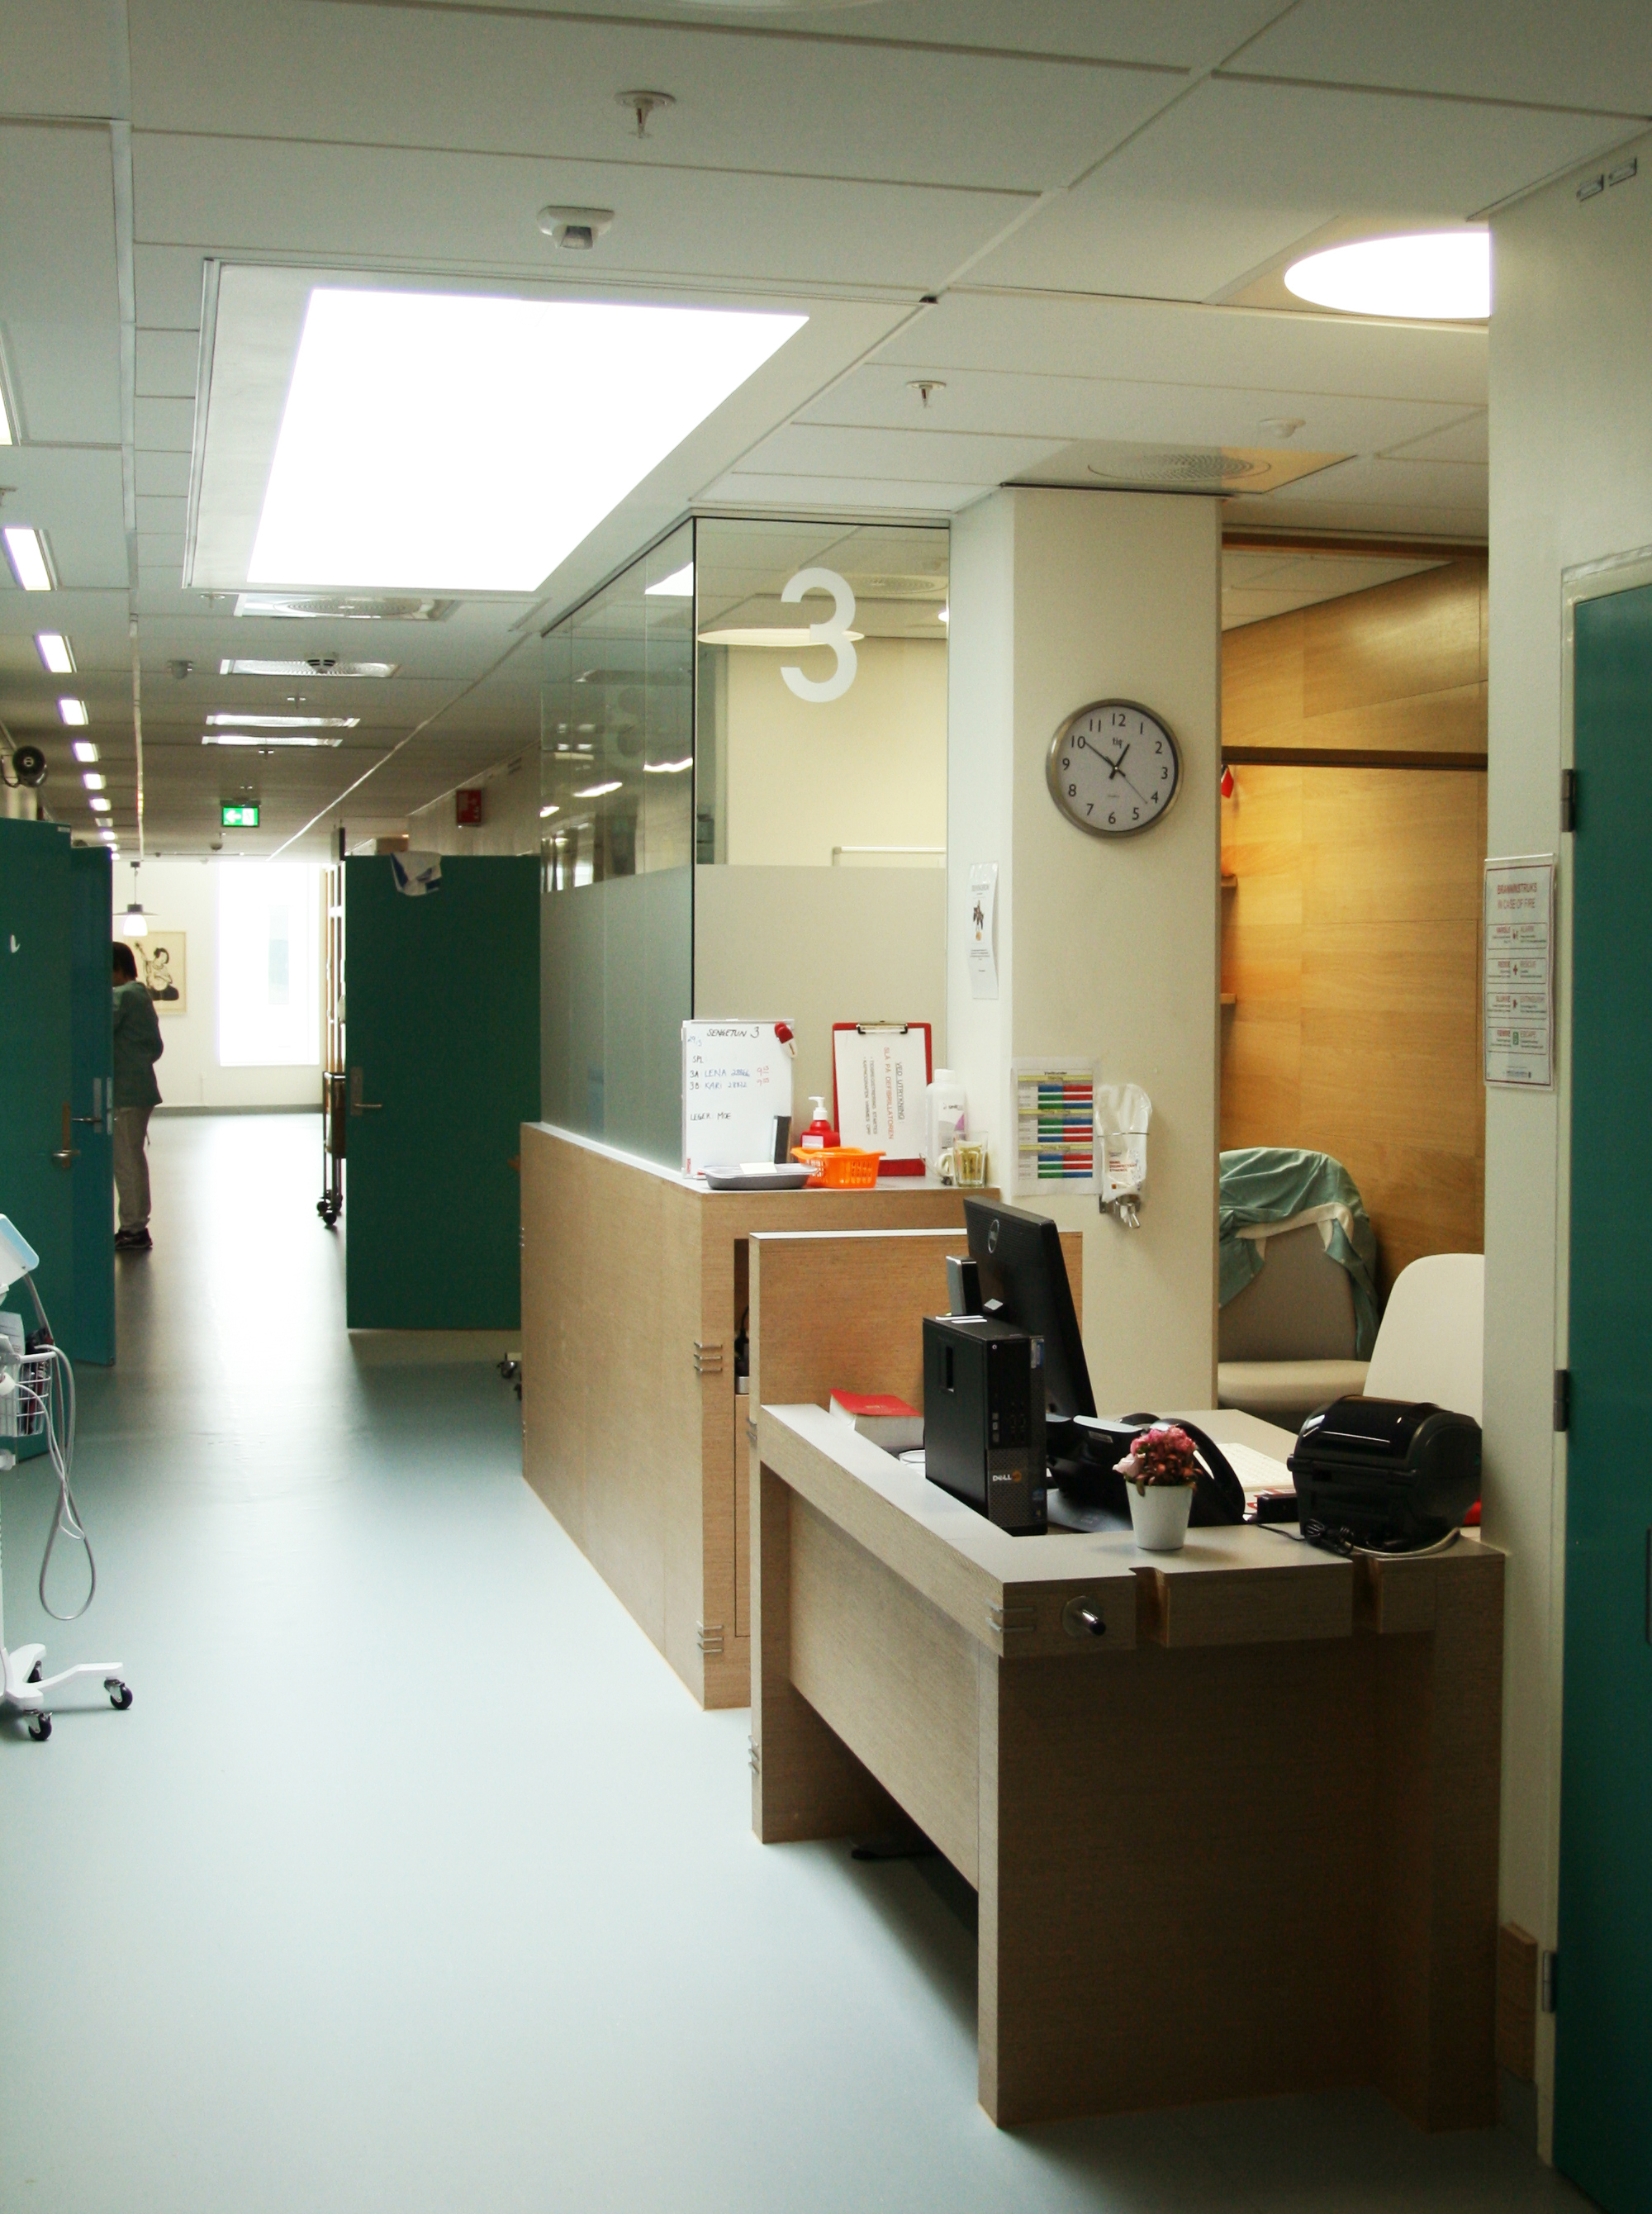
\includegraphics[scale=0.1]{A1_arbeidstasjon.jpg}
		\caption{Arbeidsstasjon på sengetun slik den er på avdeling A1 							\citep{sykehuskart}}
		\label{fig:A1_arbeidsstasjon}
	\end{subfigure}
\caption{Arbeidsstasjon på sengetun}
\label{fig:arbeidsstasjon}
\end{figure}

\section{System}
Pasientsignalsystemet består av et fast og et trådløst system. Det faste systemet består av anropspanel, rompanel og vaktromsapparat, mens det trådløse består av IP-telefoner, pasientterminaler og PC'er som kjører pasientsignalapplikasjon. En overordnet oversikt over varslingen av pasientsignal er illustrert i figur \ref{fig:detteskjer}. En mer detaljert beskrivelse finnes i vedlegg \ref{chp:appendix_dagenssystem}.

\begin{figure}[H]
\centering
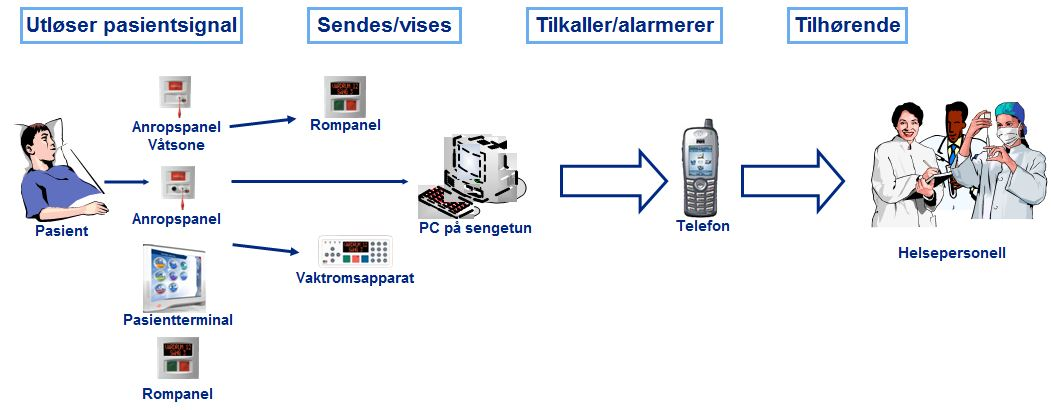
\includegraphics[scale=0.5]{alarmprosess.jpg}
\caption{Dette skjer ved utløst pasientsignal.}
\label{fig:detteskjer}
\end{figure}

\noindent
Hver arbeidsstasjon har en PC som kjører pasientsignalapplikasjonen, og gjennom denne kan sykepleierne registrere seg i en bemanningsplan (figur \ref{IMATISbemanningsplan}) og får oversikt over hvilke rom som er tilstedemarkert eller har pågående pasientsignaler og hasteanrop (figur \ref{IMATISpasientapplikasjon}). Bemanningsplanen gir pleierne mulighet til å selv påvirke hvordan pasientsignalene skal distribueres. Pleiere har mulighet til å registrere seg som primær og/eller disponibel på pasientrom og som disponibel på hele sitt eget eller andre tun. Det faste systemet er konfigurert i fysiske, kablede sløyfer som kobler sammen sengetun og gjør det mulig å motta varslinger fra andre tun på veggpanelene. I tilfeller hvor man ønsker å motta signaler fra tun som er koblet til andre sløyfer må pleierne motta disse på sin telefon, da dette kan konfigureres gjennom bemanningsplanen. Et utløst pasientsignal vil først varsles på telefon til den pleieren som er registrert som primær på det aktuelle rommet. Dersom signalet ikke blir godtatt vil det gå videre til disponible pleiere. Signalet vil fortsette i denne løkken til det blir besvart.

\begin{figure}[H]
\centering
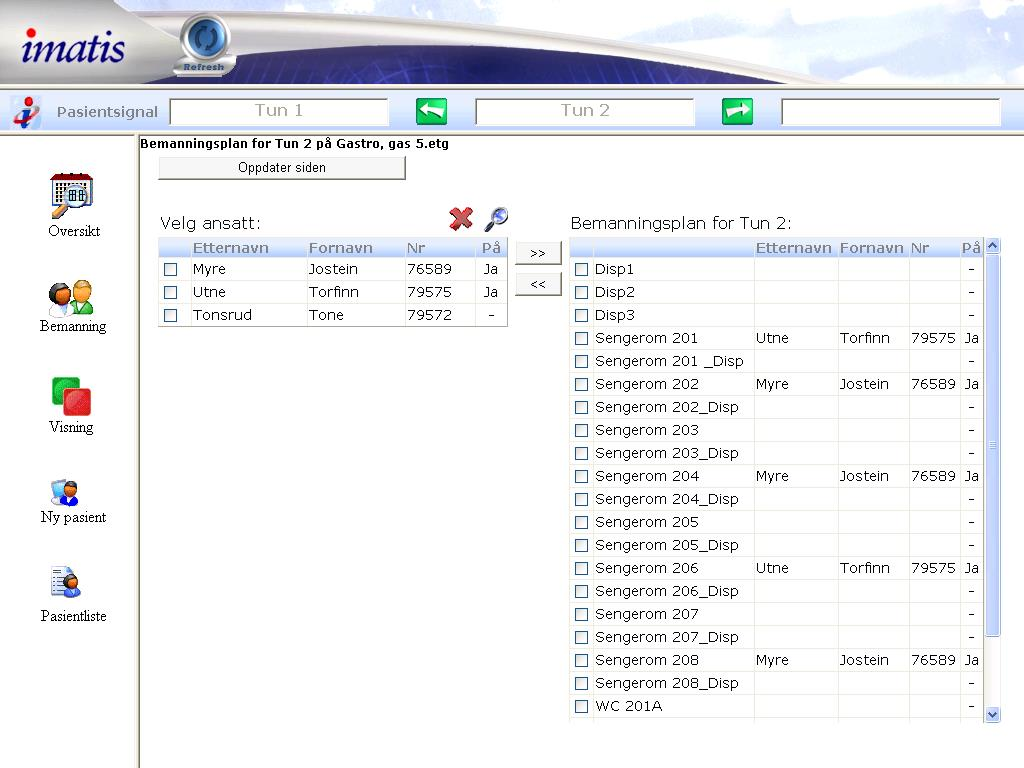
\includegraphics[scale=0.4]{bemanningsplan.jpg}
\caption{Bemanningsplan}
\label{IMATISbemanningsplan}
\end{figure}

\begin{figure}[H]
\centering
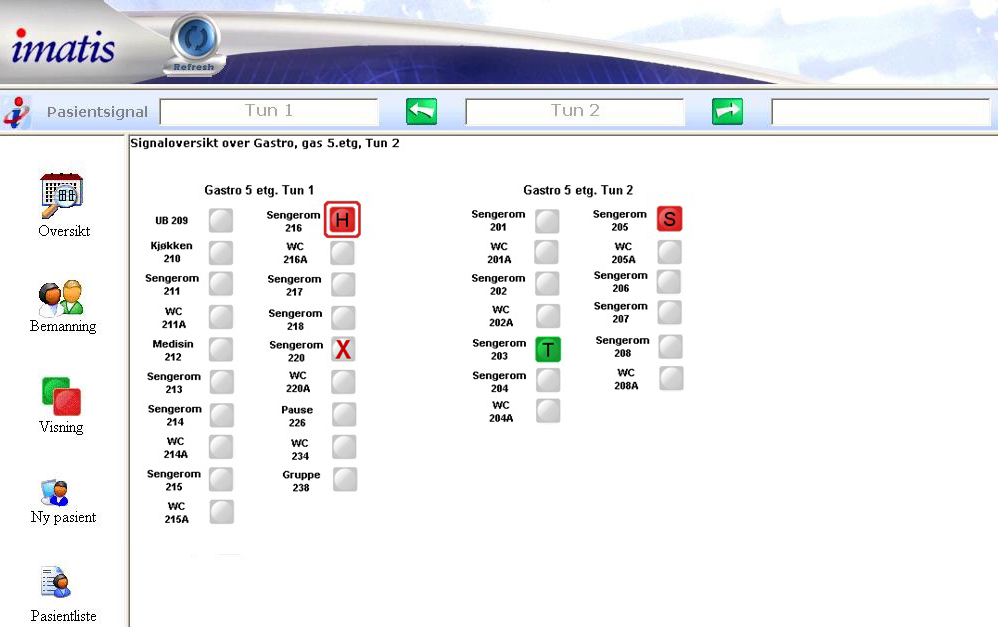
\includegraphics[scale=0.4]{pasientapplikasjon.jpg}
\caption{Signaloversikt på IMATIS-skjerm}
\label{IMATISpasientapplikasjon}
\end{figure}

\noindent
Pasientene kan tilkalle sykepleier ved å blant annet trekke i snoren på anropspanelet som er montert på veggen ved sengen. Signalet varsles da via vaktromsapparatet som henger synlig på sengetunet, via rompaneler på de pasientrom hvor sykepleiere er tilstedemarkert (denne markeringen gjøres ved at sykepleier trykker på den grønne knappen på rompanelet) og på telefonen til sykepleiere i henhold til bemanningsplanen (figur \ref{varslinger}). 

\begin{figure}[H]
        \centering
         \begin{subfigure}[b]{0.3\textwidth}
        		\centering
                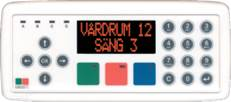
\includegraphics[scale=1.1]{vaktromsapparat.jpg}
                \caption{Vaktromsapparat}
                \label{rompanel}
        \end{subfigure}
        \begin{subfigure}[b]{0.3\textwidth}
        		\centering
                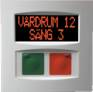
\includegraphics[scale=1.8]{rompanel.jpg}
                \caption{Rompanel}
                \label{rompanel}
        \end{subfigure}
          \begin{subfigure}[b]{0.3\textwidth}
        		\centering
                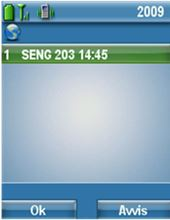
\includegraphics[scale=0.6]{signal_telefon.jpg}
                \caption{Telefon}
                \label{signal_telefon}
        \end{subfigure}      
        \caption{Varslinger av pasientsignal}
        \label{varslinger}
\end{figure}

\noindent
Ved et innkommende pasientsignal kan sykepleieren velge å godta eller avvise signalet på telefonen (figur \ref{signal_telefon}). Dersom pleieren velger å avvise signalet, eller ingen valg gjøres innen 15 sekunder, sendes signalet videre til neste pleier i henhold til bemanningsplanen. Dersom pleierne velger å godta signalet blir dette lagt i arbeidslisten på telefonen, og pleieren har 120 sekunder på seg til å tilstedemarkere seg på det aktuelle pasientrommet \citep{BrukermanualforPasientsignalogPasientsignalapplikasjon}. 

\noindent
Pleiere kan utløse hasteanrop i tilfeller hvor de har behov for assistanse. Dersom pasientrommet er tilstedemarkert gjøres dette ved å trykke på den røde knappen på rompanelet, hvis ikke må denne holdes inne i to sekunder \citep{BrukerveiledningforPasientsignal}.

\noindent
Der de samme signalene varsles på veggpanelene og på telefon fører en forsinkelse i det trådløse systemet til at signalet varsles tidligere på veggpanelene. Det foreligger desverre ingen tall på hvor stor forsinkelsen er. 

\noindent
Systemet skiller seg fra det som ble brukt tidligere, blant annet i at pasientsignal da kun ble varslet på paneler på vegg og på større paneler i taket (se figur \ref{takpanel}). Også knappen sykepleierne brukte for å formidle behov for assistanse ble fjernet (figur \ref{assistanseknapp_gammel}). 

\begin{figure}[H]
        \centering
        \begin{subfigure}[b]{1.0\textwidth}
        		\centering
                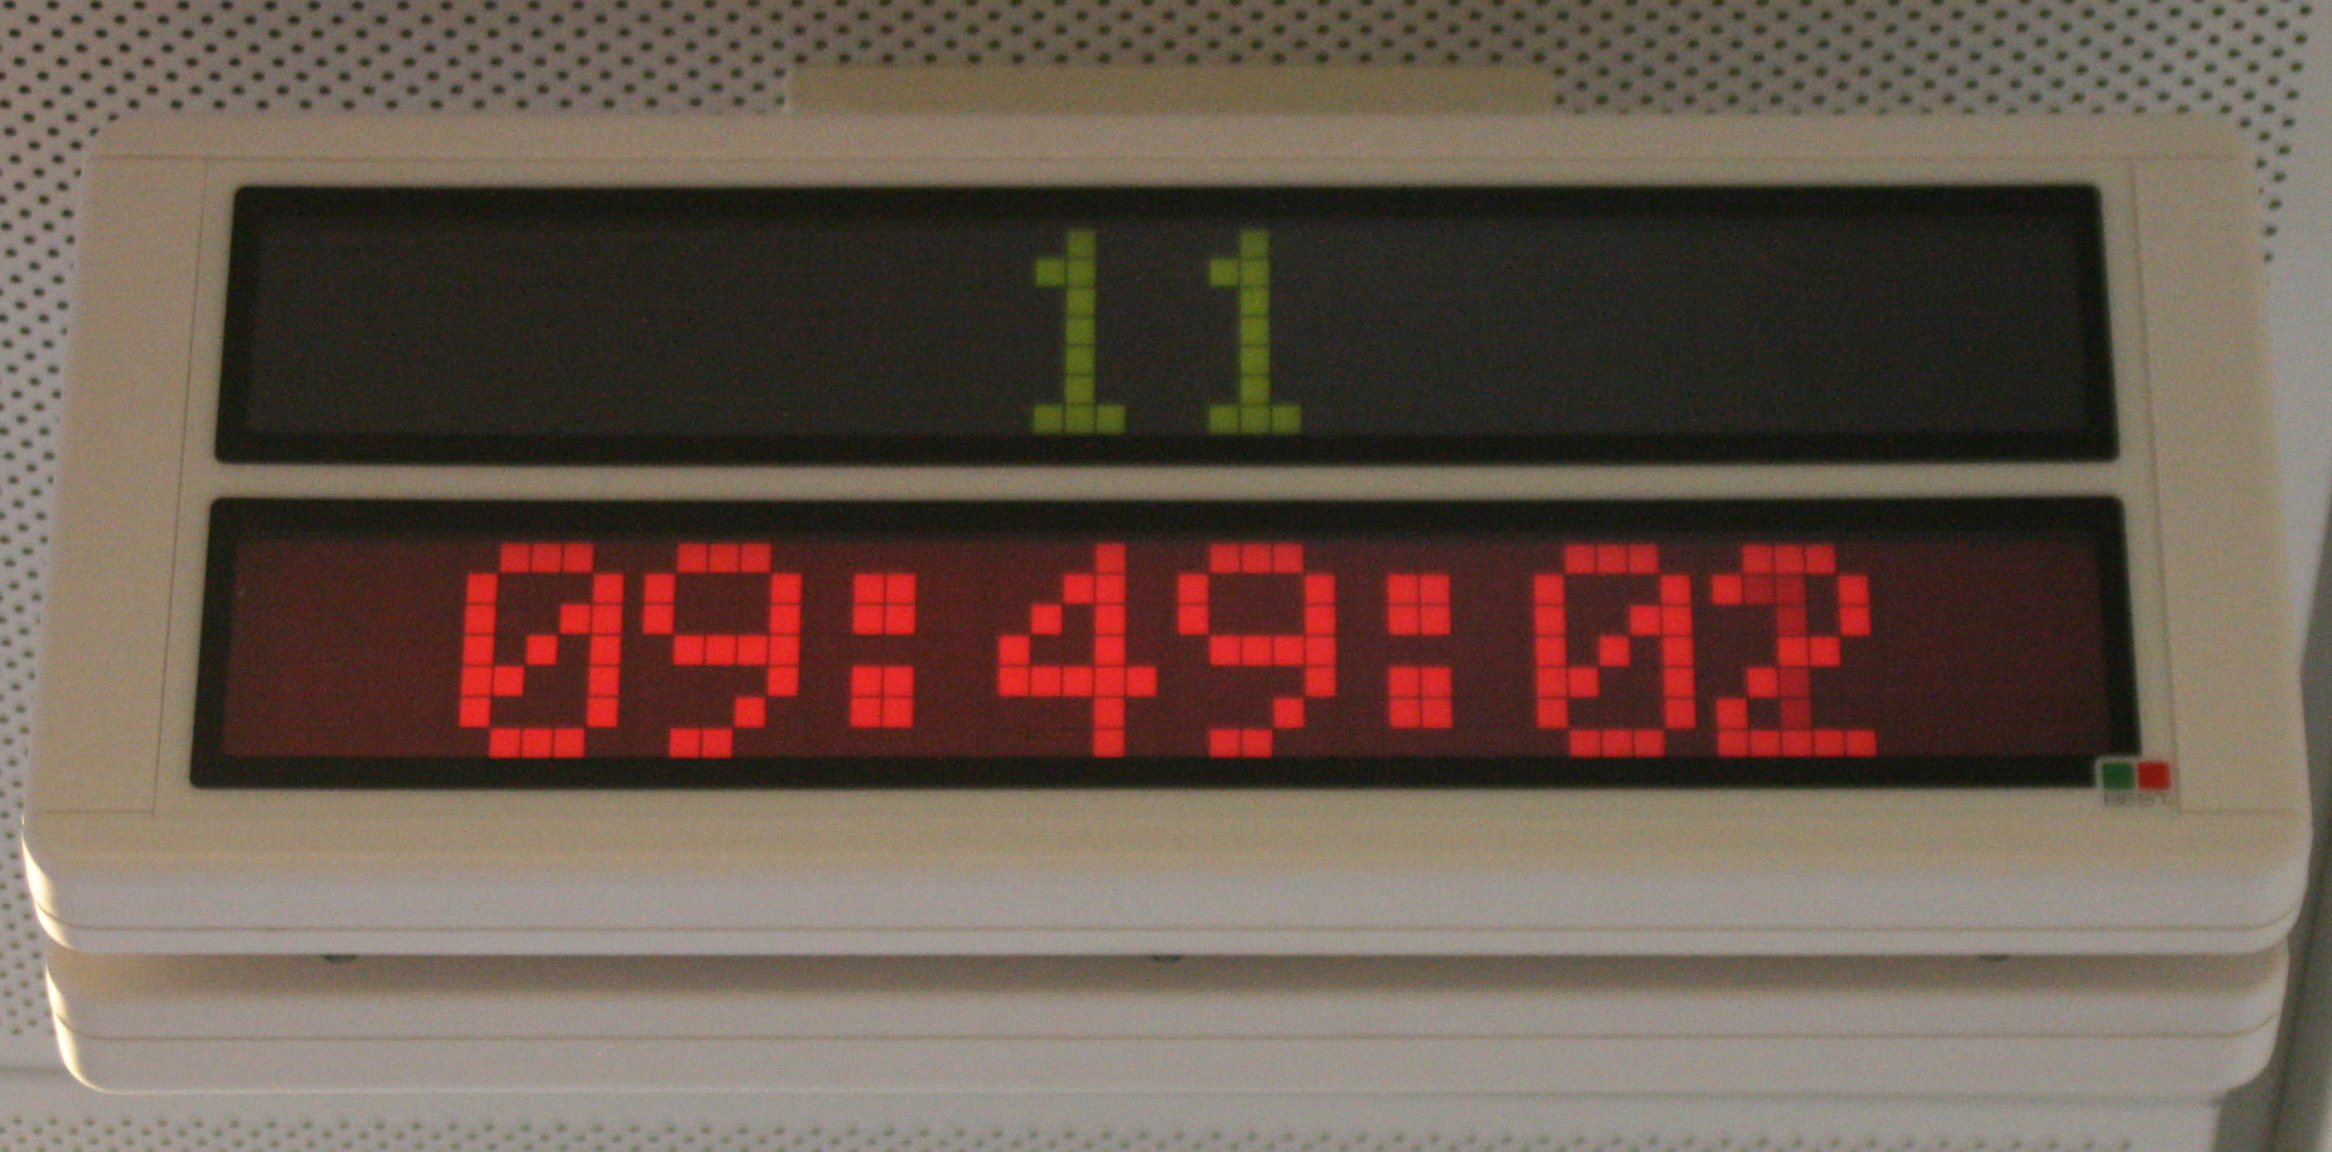
\includegraphics[scale=0.5]{takpanel.jpg}
                \caption{Panel i taket slik det var på det gamle sykehuset}
                \label{takpanel}
        \end{subfigure}
        
        \begin{subfigure}[b]{1.0\textwidth}
        		\centering
                
\includegraphics[scale=0.08]{assistanseknapp.jpg}
                \caption{Rompanel med egen knapp for assistansesignal}
                \label{assistanseknapp_gammel}
        \end{subfigure}
        \caption{Features ved det gamle sykehuset}
        \label{takass}
\end{figure}


\noindent
I forkant av innflyttingen fikk de ansatte opplæring i hvordan det nye pasientsignalsystemet fungerte. Noen fikk mer omfattende opplæring og ble $"$superbrukere$"$, med den hensikt å fungere som ambassadører for systemet og hjelpe til med opplæring på avdelingene. Den første tiden etter at systemet var tatt i bruk var det også plassert $"$on site help desk$"$ på alle avdelinger for å svare på spørsmål og hjelpe til med bruk. I dag er det den enkelte avdeling som har ansvar for opplæring av sine nyansatte. 

\noindent
Ved innflyttingen i nytt sykehus var det meningen at alle skulle bruke telefonen til å motta pasientsignaler. Det var derimot noen avdelinger, deriblant avdeling A1, som viste sterk motstand og ikke ønsket å bruke telefonene til dette.
Høsten 2013 flyttet avdelingen på nytt inn i nye lokaler, og gikk i forbindelse med dette med på å bruke systemet slik det var tiltenkt i en prøveperiode på 14 dager. Etter denne prøveperioden gikk avdelingen likevel tilbake til å ikke motta pasientsignaler på telefon. I forbindelse med denne flyttingen fikk de også tilbake assistanseknappen (figur \ref{assistanseknapp_ny}) de lenge hadde ønsket seg. Denne er plassert på et eget panel over rompanelet inne på pasientrommet. Disse signalene varsles kun i det faste systemet og har en egen varslingslyd.

\begin{figure}[H]
\centering

\includegraphics[scale=0.08]{assistanseknapp.jpg}
\caption{Panel med egen knapp for assistansesignal}
\label{assistanseknapp_ny}
\end{figure}


